\subsubsection{\textit{Histograma}}

De tal forma, dando continuidade ao assunto, o histograma é um método que auxilia na identificação de objetos e/ou características específicas da imagem, obtendo uma maior precisão nos resultados obtidos.

Segundo \citeonline{FILHO1999}, histograma são conjuntos de vários números no qual são indicados os percentuais de \textit{pixels} de uma imagem que possui determinados níveis de cinza. Estes valores, normalmente representados por gráficos, apresentam, para cada nível de cinza, o seu percentual de \textit{pixels} correspondente na imagem. Com base nessa análise feita pelo histograma, pode-se obter os níveis de contraste, brilho, e ate mesmo informações de predominância clara ou escura.

\citeonline{FILHO1999} explicam que, através de equações matemáticas, é possível obter um resultado satisfatório ao analisar cada elemento deste conjunto. Este trabalho não tem por finalidade apresentar e/ou explicar cálculos matemáticos que cada função executa.

De forma a complementar o assunto, \citeonline{MAIZA2013} expressa em sua tese que, ao obter o histograma da imagem, pode-se alcançar medidas estatísticas dos níveis de cinza da imagem, como por exemplo o seu valor mínimo e máximo, valor médio, variância e desvio padrão. Portanto, o histograma seria como um método de probabilidade, onde o número de \textit{pixels} de um determinado nível de cinza pode ser utilizado para calcular um outro \textit{pixel} com o mesmo valor de cinza na imagem (\autoref{fig_histograma}).

\begin{figure}[h]
	\caption{\label{fig_histograma}Imagem (a) e seu respectivo histograma (b).}
	\begin{center}
		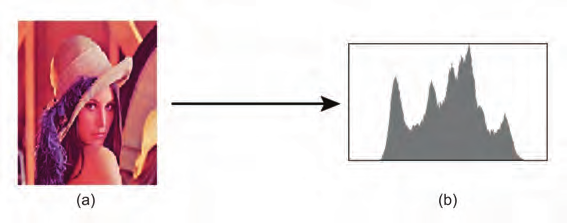
\includegraphics[scale=0.5]{4-Conteudo-Bibliografico/2-Visao-Computacional/Imagens-Visao-Computacional/histograma.png}
	\end{center}
	\centering \legend{Fonte: \citeonline{MAIZA2013}}
\end{figure}